\documentclass[tikz,border=4pt]{standalone}
% Shared style for every figure and for the deck: one accent, one
% highlight, thin lines, rounded nodes, nothing decorative.
\usepackage[T1]{fontenc}
\usepackage{lmodern}
\renewcommand{\familydefault}{\sfdefault}
\usepackage{tikz}
\usetikzlibrary{arrows.meta,positioning,calc,shapes.misc,fit,backgrounds,decorations.pathreplacing}
\definecolor{ink}{RGB}{40,40,40}
\definecolor{soft}{RGB}{150,150,150}
\definecolor{faint}{RGB}{225,225,225}
\definecolor{accent}{RGB}{0,95,115}
\definecolor{accentlight}{RGB}{214,232,236}
\definecolor{warn}{RGB}{196,84,40}
\definecolor{warnlight}{RGB}{247,226,216}
\tikzset{
  every picture/.style={color=ink, line width=0.5pt, font=\small},
  node distance=12mm and 18mm,
  box/.style={draw=ink, rounded corners=2pt, fill=white, inner sep=5pt, minimum height=7mm, align=center},
  maker/.style={box, minimum width=18mm},
  cat/.style={box, inner sep=3.5pt, minimum height=6mm},
  root/.style={box, fill=accentlight, draw=accent},
  bad/.style={box, fill=warnlight, draw=warn},
  ghost/.style={box, draw=soft, text=soft, dashed},
  flow/.style={-{Stealth[length=4pt,width=3.5pt]}, line width=0.5pt},
  sub/.style={-{Stealth[length=4pt,width=3.5pt]}, line width=0.5pt, color=soft},
  strong/.style={flow, color=accent, line width=0.8pt},
  wrong/.style={flow, color=warn},
  lbl/.style={font=\footnotesize, text=ink, inner sep=1.5pt, fill=white},
  note/.style={font=\footnotesize, text=soft, align=center},
  rate/.style={font=\footnotesize, text=accent, inner sep=1pt, fill=white},
}

\usepackage{amsmath}
\usepackage{pgfplots}
\pgfplotsset{compat=1.17}

\begin{document}
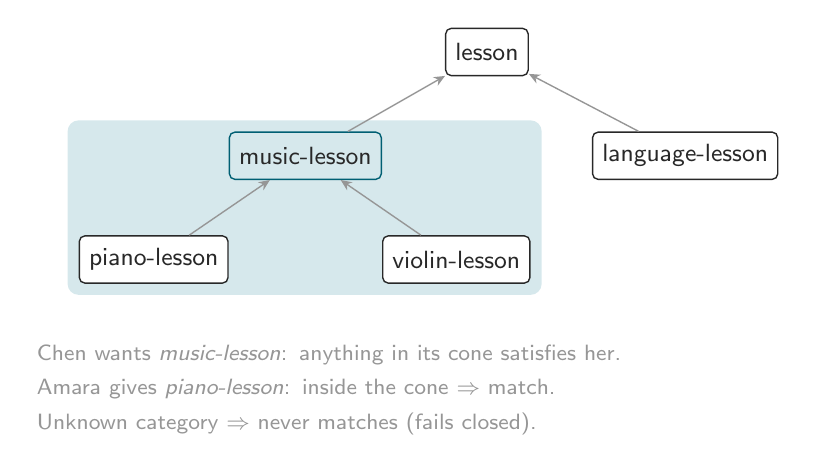
\begin{tikzpicture}[node distance=7mm and 8mm]
  \node[cat] (lesson) {lesson};
  \node[cat, below left=of lesson, fill=accentlight, draw=accent] (music) {music-lesson};
  \node[cat, below right=of lesson] (lang) {language-lesson};
  \node[cat, below left=7mm and 0mm of music] (piano) {piano-lesson};
  \node[cat, below right=7mm and 0mm of music] (violin) {violin-lesson};
  \draw[sub] (music) -- (lesson); \draw[sub] (lang) -- (lesson);
  \draw[sub] (piano) -- (music); \draw[sub] (violin) -- (music);
  \begin{scope}[on background layer]
    \node[fit=(music)(piano)(violin), rounded corners=4pt, fill=accentlight, inner sep=4pt] (cone) {};
  \end{scope}
  \node[note, below=5mm of cone.south, text width=96mm, align=left, anchor=north, xshift=14mm] {Chen wants \emph{music-lesson}: anything in its cone satisfies her.\\[3pt] Amara gives \emph{piano-lesson}: inside the cone $\Rightarrow$ match.\\[3pt] Unknown category $\Rightarrow$ never matches (fails closed).};
\end{tikzpicture}
\end{document}
